\documentclass[a4paper, 12pt]{article}

\usepackage[utf8]{inputenc}
\usepackage{amsmath}
\usepackage[]{amsfonts}
\usepackage[]{graphicx}
\usepackage[]{amsthm}

\title{CS231A Course Notes 2: Single View Metrology}
\author{Kenji Hata and Silvio Savarese}
\date{}


\renewcommand\emph{\textbf}

\begin{document}

\maketitle

\section{Introduction}
In the previous lecture notes, we discussed how we can transform points from the real, 3D world into digital images using the extrinsic and intrinsic properties of cameras. We looked at how we can use known structure in a calibration rig and its corresponding image to deduce these camera properties. This time, we will look at a related problem: can we recover known structure of the 3D world if we have a single image and know the properties of the camera that took the image? We will then more generally discuss what information can be deduced from a single image.

\section{Transformations in 2D}
To better understand how we can learn from images, we should be able to first know about the various transformations in 2D space. 

\emph{Isometric transformations} are transformations that preserve distances. In its most basic form, an isometry can be described as a rotation $R$  and translation $t$. Therefore, mathematically, they are defined as
\begin{equation*}
    \begin{bmatrix}x'\\y'\\1\end{bmatrix} = \begin{bmatrix}R & t\\ 0 & 1\end{bmatrix}\begin{bmatrix}x\\y\\1\end{bmatrix}
\end{equation*}
where $\begin{bmatrix}x'&y'&1\end{bmatrix}^T$ is the point achieved after the isometric transformation. 

\emph{Similarity transformations} are transformations that preserve shape. Intuitively, they can do everything that isometric transformations can plus scaling. Mathematically, they are denoted as 
\begin{equation*}
    \begin{bmatrix}x'\\y'\\1\end{bmatrix} = \begin{bmatrix}SR & t\\ 0 & 1\end{bmatrix}\begin{bmatrix}x\\y\\1\end{bmatrix},\ S = \begin{bmatrix}s & 0\\ 0 & s\end{bmatrix}
\end{equation*}
Since they preserve shapes, they also preserve ratio of lengths and angles. Note that every isometric transformation is a specific form of a similarity transformation when $s=1$. The converse does not hold true however.

\emph{Affine transformations} are transformations that preserve points, straight lines, and parallelism. For some vector $v$, an affine transformation $T$ is defined as 
\begin{equation*}
    T(v) = Av + t
\end{equation*}
where $A$ is a linear transformation of $\mathbb{R}^n$. In homogeneous coordinates, affine transformations are often written as
\begin{equation*}
    \begin{bmatrix}x'\\y'\\1\end{bmatrix} = \begin{bmatrix}A & t\\ 0 & 1\end{bmatrix}\begin{bmatrix}x\\y\\1\end{bmatrix}
\end{equation*}
From the above equation, it is easy to see that all similarities (and thus isometries) are a specific case of affinities.

\emph{Projective transformations} or \emph{homographies} are any transformations that maps lines to lines, but does not necessarily preserve parallelism. In homogeneous coordinates, projective transformations are represented as
\begin{equation*}
    \begin{bmatrix}x'\\y'\\1\end{bmatrix} = \begin{bmatrix}A & t\\ v & b\end{bmatrix}\begin{bmatrix}x\\y\\1\end{bmatrix}
\end{equation*}
We see that the form is a further generalization of affine transformations, as extra degrees of freedom are added with the addition of $v$. 

Despite not preserving parallelism, projective transformations does preserve collinearity of points, as it maps lines to lines. Furthermore, we prove that the cross ratio of four collinear points remains invariant under projective transformations. The cross ratio takes four points $P_1, P_2, P_3, P_4$ on a line and computes
\begin{equation}
    \mathrm{cross\ ratio} = \frac{\|P_3-P_1\|\|P_4-P_2\|}{\|P_3-P_2\|\|P_4-P_1\|}
\end{equation}
We leave proving the invariance of the cross ratio under projective transformation as a class exercise.

\section{Points and Lines at Infinity}
Lines are important for determining structure in images, so knowing their definitions in both 2D and 3D is essential. A line in 2D can be represented with the homogeneous vector $\ell = \begin{bmatrix}a & b & c \end{bmatrix}^T$. The ratio $-\frac{a}{b}$ captures the slope of the line and the ratio $-\frac{c}{b}$ captures the y-intercept. Formally, 2D lines are defined by:
\begin{equation}
\forall p = \begin{bmatrix}x\\y\end{bmatrix} \in \ell,\ \  \begin{bmatrix}a & b & c\end{bmatrix}\begin{bmatrix}x\\y\\1\end{bmatrix} = 0
\end{equation}

In general, two lines $\ell$ and $\ell'$ will intersect at a point $x$. This point is defined as the cross product between $\ell$ and $\ell'$.

\begin{proof} 
    Given two intersecting lines $\ell$ and $\ell'$, the intersection point $x$ should lie on both lines $\ell$ and $\ell'$. Therefore, $x^T \ell = 0$ and $x^T\ell' = 0$. If we set $x = \ell \times \ell'$, then by definition of cross product, the vector $x$ is orthogonal to both vectors $\ell$ and $\ell'$. By the definition of orthogonality, $x^T \ell = 0$ and $x^T\ell' = 0$. Thus, this definition of $x$ satisfies the constraints. 
\end{proof}

What about the case of parallel lines? Everyday knowledge expects these lines to never intersect. However, this definition could be rewritten to say that these lines intersect at infinity. In homogeneous coordinates, a point at infinity is written as $\begin{bmatrix}x & y & 0\end{bmatrix}^T$. Recall the Euclidean coordinates are gathered by dividing all coordinates by the last coordinate. In this case, the coordinate is zero, achieving a point at infinity. Therefore, homogeneous coordinates give a good formulation of determining intersections, even in cases of parallel lines.

Now, let's consider two parallel lines $\ell$ and $\ell'$. When two lines are parallel, their slope is equal and thus $\frac{a}{b} = \frac{a'}{b'}$. If we compute the point of intersection using homogenoous coordinates, then we verify that
\begin{equation}
\ell \times \ell' \propto \begin{bmatrix}b \\ -a \\ 0  \end{bmatrix}= x_\infty
\end{equation}

Thus, we confirmed our intuition that two parallel lines intersect at infinity. The point of intersection at infinity of two parallel lines is also called an \emph{ideal point}. One interesting property of a point at infinity is that all parallel lines with the same slope $-\frac{a}{b}$ pass through the ideal point as shown below:
\begin{equation}
\ell ^T x_\infty = \begin{bmatrix}a & b & c\end{bmatrix} \begin{bmatrix}b \\ -a \\ 0\end{bmatrix} = 0
\end{equation}

\begin{figure}[h!]
\centering
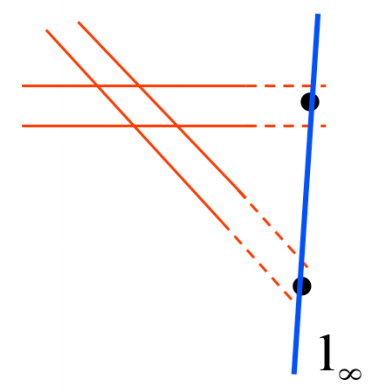
\includegraphics[width=0.5\textwidth]{figures/line_infinity.png}
\caption{Points at infinity form lines at infinity.}
\label{fig:line_infinity}
\end{figure}

The concept of points of infinity can be extended to define \emph{lines at infinity}. Consider two or more pairs of parallel lines. Each pair of parallel lines intersects at a point at infinity $\{x_{\infty,1},...,x_{\infty,n}\}$.The line $\ell_\infty$ that passes through all these points at infinity must satisfy $\forall i, \ell_\infty^T x_{\infty,i}= 0$. This means that $\ell_\infty = \begin{bmatrix}0 & 0 & c\end{bmatrix}^T$. Since $c$ is an arbitrary value, we can simple define $\ell_\infty = \begin{bmatrix}0 & 0 & 1\end{bmatrix}^T$.

If we apply a generic projective transformation $H$ to a point at infinity $p_\infty$, what will happen? 
\begin{equation}
p' =Hp_\infty = \begin{bmatrix} A &t \\ v&b \end{bmatrix}\begin{bmatrix}1\\1\\0\end{bmatrix} = \begin{bmatrix}p'_x\\ p'_y\\p'_z\end{bmatrix}
\end{equation}

Notice that the last element of $p'$ may become non-zero, which suggests that a projective transformation generally maps points at infinity to points that are no longer at infinity. However, this is not the case for affine transformations, which map points at infinity to points at infinity:
\begin{equation}
p' =Hp_\infty = \begin{bmatrix} A &t \\ 0&1 \end{bmatrix}\begin{bmatrix}1\\1\\0\end{bmatrix} = \begin{bmatrix}p'_x\\ p'_y\\0\end{bmatrix}
\end{equation}

Now let's apply a projective transformation $H$ to a line $\ell$ to get a new line $\ell'$. All points $x$ that pass through a line must satisfy the property $x^T\ell = 0$. In the transformed space, we know that lines still map to lines, which means that $x'\ell' = 0$. We can use the identity property to get \[x^TI\ell = x^TH^T H^{-T} \ell = 0\]If we apply a projective transformation to the line, then all the points become transformed as well, giving $x' = Hx$. Thus we get $x^TH^T H^{-T} \ell = x'^T\ell'$, and we find the projective transformation of a line is $\ell' = H^{-T}\ell$. Similar to our observations with points at infinity, we find that the projective transformation of a line at infinity does not necessarily map to another line at infinity. Additionally, affine transformations still map lines at infinity to lines at infinity.

\section{Vanishing Points and Lines}
So far, we have introduced the concepts of lines and points at infinity in 2D. Let us now introduce the equivalent concepts for 3D in its corresponding homogeneous coordinates. 

In the 3D world, we are now introduced to the concepts of planes. We can represent a plane as a vector $\begin{bmatrix}a&b&c&d\end{bmatrix} ^T$, where $(a,b,c)$ form a normal vector and $d$ is the distance from the origin to the plane in that normal vector's direction. Formally, a plane is defined as all the points $x$ which satisfy
\begin{equation}
x^T\begin{bmatrix}a\\b\\c\\d\end{bmatrix} = ax_1 + bx_2 + cx_3 + d = 0
\end{equation}
Lines in 3D are defined as the intersection of two planes. Since they have four degrees of freedom (a defined intercept location and slopes in each of the three dimensions), they are difficult to represent nicely in 3D space. Please see Section 3.2.2 of the Hartley \& Zisserman textbook for more details.

Points, however, are defined similarly in 3D as they are in 2D. Points at infinity in 3D are again defined as the intersection point of parallel lines in 3D. Furthermore, if we apply a projective transformation to one of these points at infinity $x_\infty$, then we obtain a point $p_\infty$ in the image plane, which is no longer at infinity in homogeneous coordinates. This point $p_\infty$ is known as a \emph{vanishing point}. But, what can we do with vanishing points?

We can derive a useful relationship between parallel lines in 3D, their corresponding vanishing point in the image, and the camera parameters $K,R,T$. Let us define $d = (a,b,c)$ as the direction of a set of 3D parallel lines in the camera reference system. These lines intersect to a point at infinity and the projection of such a point in the image returns the vanishing point $v$, which is defined by
\begin{equation}
v = Kd
\end{equation}
We leave the derivation of the above equation as an exercise. This equation can be rewritten to extract the direction $d$: 
\begin{equation}
d = \frac{K^{-1}v}{\|K^{-1}v\|}
\end{equation}

If we consider a plane $\Pi$ as a superset of parallel lines, each set of parallel lines intersects at a point at infinity. The line that passes through such set of points at infinity is the line at infinity $\ell_\infty$ associated to $\Pi$. A line at infinity is also defined as the line where two parallel planes intersect. The projective transformation of $\ell_\infty$ to the image plane is no longer a line at infinity and is called the vanishing line or the \emph{horizon line} $\ell_{\mathrm{horiz}}$. The horizon line is a line that passes through the corresponding vanishing points in the image. The horizon line can be computed as 
\begin{equation}
\ell_{\mathrm{horiz}} = H_P^{-T} \ell_\infty
\end{equation}


\begin{figure}[h!]
\centering
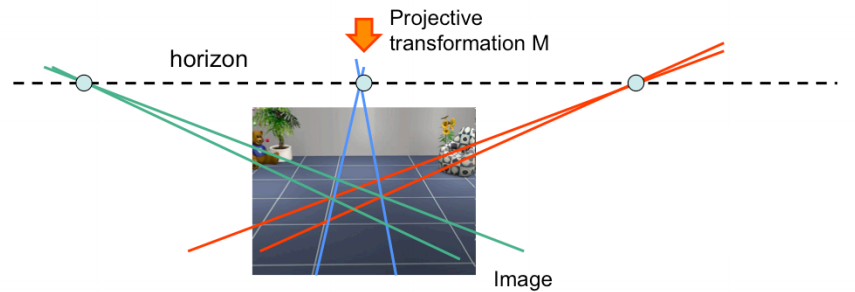
\includegraphics[width=0.8\textwidth]{figures/horizon.png}
\caption{The computed horizon line from a set of vanishing points.}
\label{fig:horizon}
\end{figure}

The concept of a horizon line allows us to answer as humans to intuitively deduce properties about the image that may not be easily apparent mathematically. For example, in Figure~\ref{fig:horizon}, although the lines on the ground are not parallel in image coordinates, we have a natural understanding that they are parallel in the 3D world.

Furthermore, the horizon line allows us to compute useful properties about the world. For example, we can derive an interesting relationship between the the normal $n$ of a plane in 3D with the corresponding horizon line $\ell_{\mathrm{horiz}}$ in an image:
\begin{equation}
n = K^T \ell_{\mathrm{horiz}}
\end{equation}
This means that if we can recognize the horizon line associated with a plane, and if our camera is calibrated, then we can estimate the orientation of that plane.
\begin{figure}[h!]
\centering
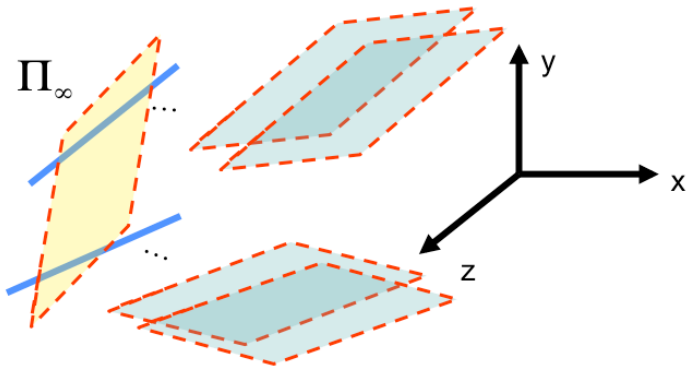
\includegraphics[width=0.8\textwidth]{figures/plane_infinity.png}
\caption{A set of two or more vanishing lines (the blue lines) defines the plane at infinity $\Pi_\infty$ (the yellow plane).}
\label{fig:plane_infinity}
\end{figure}
Before introducing the last property that relates vanishing points and lines, we first need to define the plane at infinity $\Pi_\infty$. This plane is defined by a set of 2 or more vanishing lines and is described by the vector $\begin{bmatrix} 0 & 0 & 0 &1\end{bmatrix}^T$ in homogeneous coordinates. 

\begin{figure}[h!]
\centering
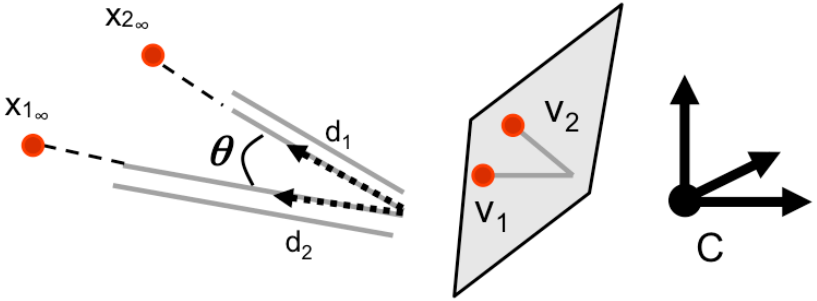
\includegraphics[width=0.8\textwidth]{figures/angles.png}
\caption{Deriving the angle between two lines.}
\label{fig:angles}
\end{figure}

The last property we introduce relates lines and planes in 3D with the corresponding vanishing points and lines in the image plane. Suppose that two pairs of parallel lines in 3D have directions $d_1$ and $d_2$, and are associated with the points at infinity $x_{1,\infty}$ and $x_{2,\infty}$. Let $v_1$ and $v_2$ be the corresponding vanishing points. Then, we find that the angle $\theta$ between $d_1$ and $d_2$ is given by using the cosine rule:
\begin{equation}
    \begin{split}
        \cos\theta &= \frac{d_1 \cdot d_2}{\|d_1\| \|d_2\|}\\
        &= \frac{v_1^T\omega v_2}{\sqrt{v_1^T \omega v_1}\sqrt{v_2^T \omega v_2}}
    \end{split}
    \label{eq:angles}
\end{equation}
where $\omega = (KK^T)^{-1}$. 

We can extend this idea further to the 3D planar case, in which we want to relate different planes in 3D. Recall that for any plane, we can compute its associated vanishing line $\ell_\mathrm{{horiz}}$ and its normal $K^T \ell_{\mathrm{horiz}}$. Therefore, we can determine the angle $\theta$ between two planes by computing the angle between each of the planes' normal vectors $n_1$ and $n_2$. We derive the angle $\theta$ between two planes with a vanishing lines $\ell_1$ and $\ell_2$ respectively:
\begin{equation}
    \begin{split}
        \cos\theta &= \frac{n_1 \cdot n_2}{\|n_1\| \|n_2\|}\\
        &= \frac{\ell_1^T\omega^{-1} \ell_2}{\sqrt{\ell_1^T \omega^{-1} \ell_1}\sqrt{\ell_2^T \omega^{-1} \ell_2}}
    \end{split}
\end{equation}

\section{A Single View Metrology Example}
\begin{figure}[h!]
\centering
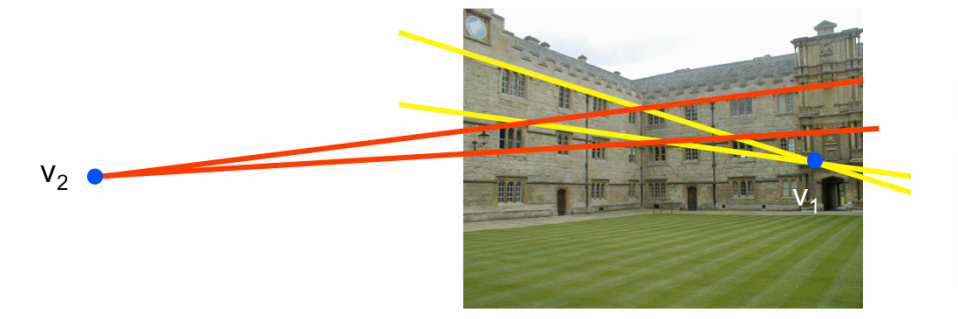
\includegraphics[width=0.8\textwidth]{figures/example1.png}
\caption{The example setup with two vanishing points for a pair of perpendicular planes.}
\label{fig:example1}
\end{figure}
Suppose that we can identify two planes in an image of the 3D world. Additionally, let's suppose that we can identify a pair of parallel lines on each of these planes. This allows us to estimate two vanishing points $v_1$ and $v_2$ in the image. Finally, let's suppose that we know that these planes are perpendicular in 3D. In this case, we know that from Equation~\ref{eq:angles}, that $v_1\omega v_2 = 0$. 

But recall that $\omega$ depends on the camera matrix $K$, which is potentially unknown at this time. Therefore, is knowing these two vanishing points sufficient for accurately estimating the camera parameters? Considering that $K$ has 5 degrees of freedom and that $v_1 \omega v_2 = 0$ provides only one constraint, we do not have enough information to calculate $K$. 
\begin{figure}[h!]
\centering
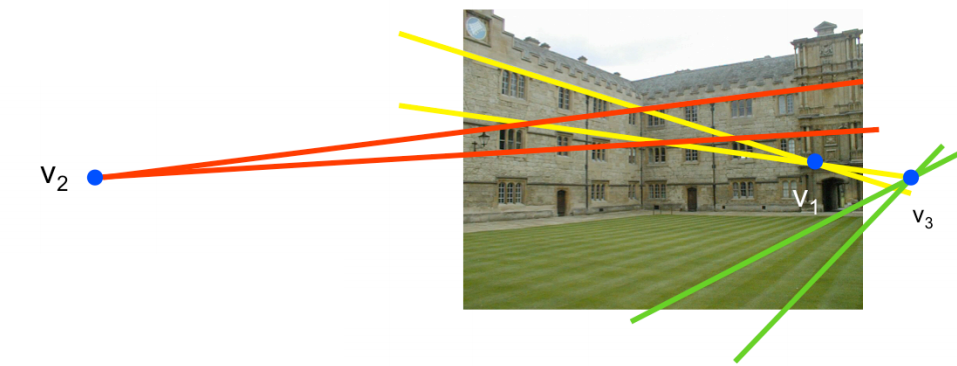
\includegraphics[width=0.8\textwidth]{figures/example2.png}
\caption{The example setup with three vanishing points for a set of mutually perpendicular planes.}
\label{fig:example2}
\end{figure}
What if we are able to find another vanishing $v_3$ for another mutually orthogonal plane? Then we know that $v_1\omega v_2 = v_1\omega v_3 = v_2\omega v_3 = 0$. Since each pair gives a constraint, we only end up with 3 out of the 5 constraints needed to compute $K$. However, if we make the assumption that the camera has zero-skew and square pixels, then we can add the additional two constraints needed. By these assumptions, then we know that $\omega$ takes on the form 
\begin{equation}
    \omega = \begin{bmatrix}\omega_1 & 0 & \omega_4 \\ 0 & \omega_1 & \omega_5 \\ \omega_4 & \omega_5 &\omega_6 \end{bmatrix}
\end{equation}

If you noticed carefully, there are four variables in the definition of $\omega$. However, we can only know $\omega$ up to scale, which reduces the amount of actual variables to three, allowing it to be solved. Once we have $\omega$, then we can use Cholesky decomposition to compute $K$. Thus, we have managed to calibrate the camera using a single image!

Once $K$ is known, then we can reconstruct the 3D geometry of the scene. For example, we can compute the orientation of all the planes identified above. Therefore, a single image can be readily used to uncover a wealth of information about the scene it captures.

\end{document}
